\section{Method} \label{sec:method}
The optimization of power regulation while minimizing loads, requires a model that can predict the power output and the loads of a wind farm. This section describes how this is implemented.

An overview of the optimization procedure used is illustrated in Figure \ref{fig:optim}.
The power output of a wind farm as well as the wake development in the wind farm are estimated using the FLORIS model \cite{Gebraad2016} (Section \ref{sec:floris}). Given a certain wind field the program FAST calculates bending moments. The program MLife is used to convert these bending moments into short-term Damage Equivalent Loads (DELs) \ref{sec:fast}. These DELs are precalculated for different situations and stored in a lookup table so it can be quickly retrieved during optimization (Section \ref{sec:lut}). The optimization algorithm uses a cost function that combines the DEL and power data to find the optimal wind turbine configuration that has minimal loads while tracking a predefined reference power (Section \ref{sec:optimization}).

\begin{figure*}[h]
	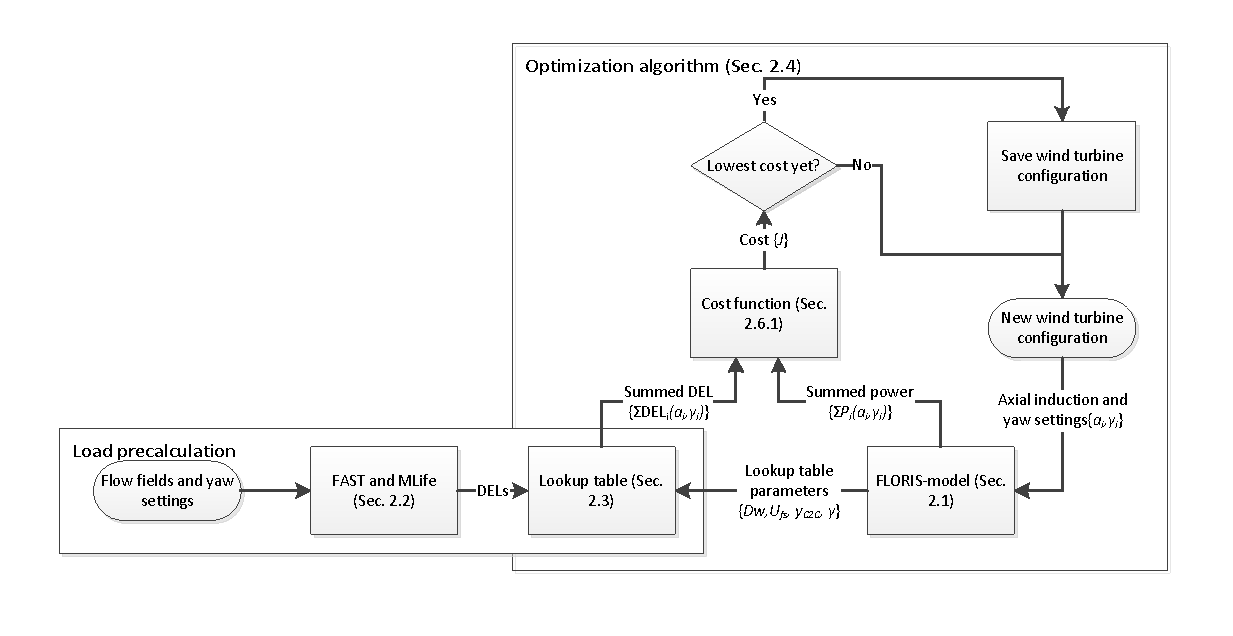
\includegraphics[width=\linewidth]{./Figures/OptimizationProcess.pdf}
	\caption{Overview of the model used in this paper. For a random wind turbine configuration the summed power and summed DEL are evaluated and used as input for the cost function. If the resulting cost is the lowest yet, the wind turbine configuration is saved. Then a new configuration is generated and the process starts again.}
	\label{fig:optim}
\end{figure*}

\subsection{FLORIS} \label{sec:floris} The FLOw Redirection and Induction in Steady state (FLORIS) model is used to simulate the wind flow in a wind farm while also generating power output data. The model is a function of the yaw misalignment and the axial induction \cite{Gebraad2016}. FLORIS is a parametric model fitted to high-fidelity data from a computational fluid dynamics simulation, making it a relatively accurate model with low computation time \cite{Dijk2016}. 

\subsubsection{Wake modelling}
\label{wakemodel}
%As can be seen in Figure \ref{fig:wake}, 
FLORIS contains a wake model which divides the wake into three different zones, as illustrated in Figure \ref{fig:wake}. These zones are denoted by $q$ and defined as the near wake ($q$=1), the far wake ($q$=2) and the mixing zone ($q$=3). Each zone has its own function for the zone diameter and wind speed, which are calculated by FLORIS using Equations \ref{eq:Dw} to \ref{eq:c}. 


\begin{figure}
  	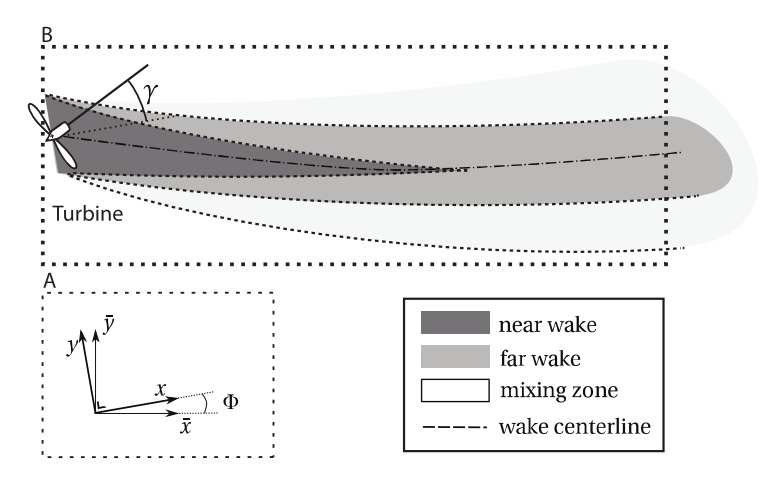
\includegraphics[width=\linewidth]{./Figures/WakeFLORIS.png}
  	\caption{Simplified top view representation of a wake of a turbine by FLORIS \cite{Gebraad2016}.}
	\label{fig:wake}
\end{figure}

The diameter of the wake zones are calculated using Equation \ref{eq:Dw}. Let the $D_i$ denote the rotor diameter of the $i${\textsuperscript{th}} turbine, $k_e$ a coefficient that describes expansion of the zones, and $m_{e,q}$, the expansion factor as used in \cite{Gebraad2016}. The x location of the turbine is denoted by $X_i$.

\begin{equation}
\label{eq:Dw}
D_{w,i,q}(x) = max({D_i + 2k_em_{e,q}([x - X_i],0} )
\end{equation}

The diameter of the third wake zone $D_{w,i,q=3}$ is frequently used further in this paper. To increase readability, this diameter will be referred to as 'wake diameter' or $D_w$. This diameter $D_w$ increases proportionally with downwind distance $x$ (for orientation see Figure \ref{fig:wake}).
The velocity in the wake is related to this downwind distance $x$ as well, see Equation \ref{eq:Uw}. Here the wake velocity is an argument of the wake decay coefficient $c_{i,q}(x)$ and the axial induction factor $a_i$. The axial induction factor is a measure for the wind speed reduction behind a turbine relative to free stream wind velocity. The wake decay coefficient $c_{i,q}(x)$ describes the decay of velocity for each wake zone and is defined in Equation \ref{eq:c}. In this equation, the coefficient $m_{U,q}$ is a parameter that defines how quickly the wake decays for the different wake zones \cite{Gebraad2016}.

\begin{equation}
\label{eq:Uw}
U_{w,i}(x) = U_i\left( {1-2a_{i}c_{i,q}(x)} \right)
\end{equation} 

\begin{equation}
\label{eq:c}
c_{i,q}(x) = \left[ \frac{D_i}{D_i + 2k_em_{U,q}(\gamma_i)[x - X_i]} \right]^2
\end{equation}



%//programming tool for the simulation of dynamic (load) responses of wind turbines (by NREL) 
%\noindent
%(klopt deze cite nog met deze benaming?),-->
\subsection{FAST \& MLife} \label{sec:fast} FAST is a dynamic turbine model \cite{Jonkman2005}. Among other things, it computes the root out of plane bending moments (RootMOops) on turbine blades. RootMOops cyclically change with the blade's orientation in the wind, which is a function of the turbine's rotation frequency. Compiling the RootMOops as a function of time results in a load spectrum.

The program MLife is used to convert these load spectra into short-term damage equivalent loads (DELs). A DEL is a constant amplitude fatigue-load, containing the same data as the load spectra do. However, all other dynamic load influencing factors are kept constant for each load spectrum. As such making it possible to compare the different load spectra \cite{Wilson2017, MLife}.


\begin{figure}
  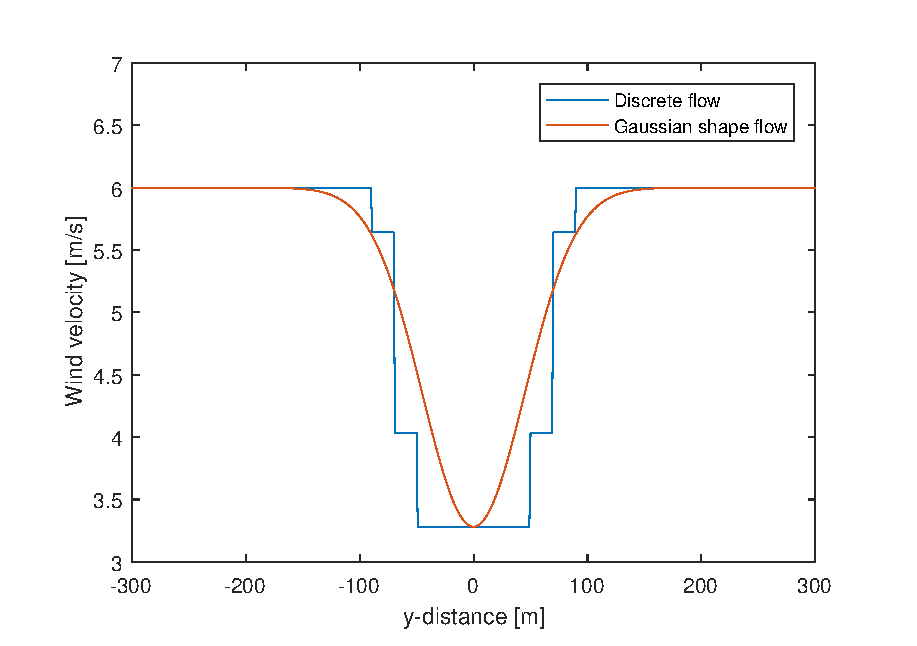
\includegraphics[width=\linewidth]{./Figures/PlotGausDiscWakeDWake180U6yaw0.eps} %Plot with Gauss vs Discr flow, Dwake = 180, u_mean = 6, yaw = 0
  \caption{Discrete wake velocity versus Gaussian wake velocity profile at a height of 90 m, hub height.} %for Dwake = 180 m, U = 6 m/s, and yaw = 0
  \label{fig:disgaus}
\end{figure}

%\noindent

\subsubsection{Flow field} \label{sec:flowfield}
A wind flow profile is used in FAST to calculate the loads. This is a 2-dimensional grid containing wind velocity data at the location of the wind turbine rotor-plane.

This study makes the wind data more realistic by implementing both a continuous wake distribution, the Gaussian distribution, as well as the natural phenomenon, wind shear.

\paragraph{Gaussian wake}
FLORIS describes a discrete flow field of a wake, with three zones as described in section \ref{wakemodel}. The flow field of the wake in FLORIS is calculated with equations (\ref{eq:Dw} to \ref{eq:c}). A wake, however, does not have these discrete zones. To create a more fluent transition between the different wake-zones, a Gaussian distribution of the flow field is introduced \cite{Bastankhah2016}. The velocity profile difference can be seen in Figure \ref{fig:disgaus}.  The Gaussian distribution is calculated as follows: 

\begin{equation}
\label{eq:gaus}
G(y, z) = A e^{-\left(\frac{y^2}{2\sigma_y} + \frac{z^2}{2\sigma_z}\right)}
\end{equation}
The amplitude of the Gaussian, $A$, is set to be equal to the velocity loss of the inner wake zone, $U_{w,1}$, as generated by FLORIS. $\sigma_y$ and $\sigma_z$ reflect the Gaussian standard deviation in horizontal and vertical direction, respectively. These standard deviations are related to the wake diameter $D_{w}$ following Equation \ref{eq:sigm}:
\begin{equation}
\label{eq:sigm}
\sigma_y,\sigma_z = \frac{D_{w}}{n} 
\end{equation}
\\
Where fit parameter $n$ can be modified to change the width of the Gaussian. Consequently, making it possible to fit a Gaussian on the wake zones of FLORIS (Figure \ref{fig:disgaus}). Future versions of FLORIS will have this Gaussian distribution implemented as well. 

\paragraph{Wind shear} \label{sec:windshear}
Another aspect added to improve the accuracy of the wind data is wind shear. This natural phenomenon is the result the earth's surface slowing the wind down closer to the ground. This results in a difference in wind speed over the height ranges of the turbine, which has a significant effect on the DELs \cite{Firtin2011}.  The velocity distribution is calculated as follows: 
\begin{equation}
\label{eq:shear}
v = v_{ref} \left(\frac{h}{h_{ref}}\right)^\alpha
\end{equation}
Here $v$ and $v_{ref}$ are the velocity at heights $h$, and $h_{ref}$  respectively. Value $\alpha$ is the wind shear coefficient which depends on different factors. The coefficient $\alpha$  reflects terrain type, and is for this paper fixed at value 0.1 representing a surface close to ocean and smooth ground \cite{Firtin2011}. Figure \ref{fig:windshear} shows the flow fields of a wake both before and after the implementation of wind shear.

\begin{figure}
	\centering
	\begin{subfigure}[b]{0.50\textwidth}
		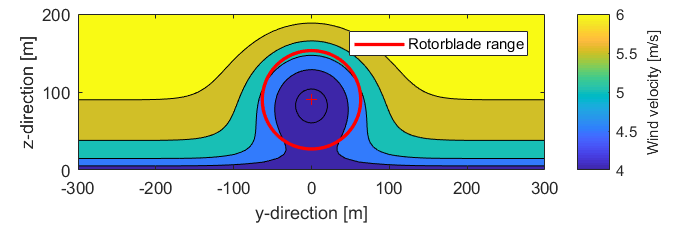
\includegraphics[width=\linewidth]{./Figures/PlotwithshearU6D220.png} %Plot with windshear u_mean = 6
		\caption{Flow field with wind shear.}
		\label{fig:windsh}
	\end{subfigure}
	
	\begin{subfigure}[b]{0.50\textwidth}
		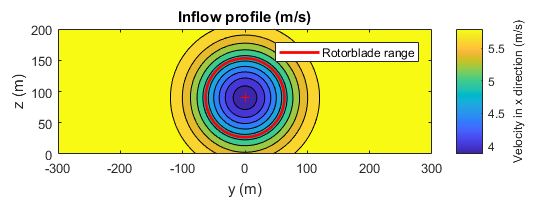
\includegraphics[width=\linewidth]{./Figures/PlotwithoutshearU6D220.png} %Plot without windshear u_mean = 6
		\caption{Flow field without wind shear.}
		\label{fig:nowindsh}
	\end{subfigure}
	
	\caption[Two Gaussian flow fields]{Gaussian wind fields with a free stream velocity of 6 $m/s$ at a height of 90 $m$. The outer diameter of de wake is 220 $m$ and the diameter of the rotor blades is 126.4 $m$.}
	\label{fig:windshear}
\end{figure}




\begin{table}[h]
	%\renewcommand{\arraystretch}{1.3} 
	\caption{Overview of the minimum value, maximum value, and step size of the parameters: diameter of the wake ($D_w$), free stream wind speed ($U_{fs}$), yaw of the turbine ($\gamma$) and the center to center distance between the center of the turbine and the center of the wake ($y_{C2C}$).}
	\centering
	\label{tab:pars}
	\begin{tabular}{lccc}
		\hline
	 	& Min & Max & Step-size \\ 
		\hline
		$D_w$ [m] & 180 & 330 & 25 \\
		$U_{fs}$ [m/s] & 6 & 8 & 2 \\
		$\gamma$ [deg] & -30 & 30 & $^*$ \\
		$y_{C2C}$ [m] & -250 & 250 & 10 \\
		\hline
	\end{tabular}

$^* \gamma$ has no constant step-size. The input values are: \{-30, -20, -10, -5, 0, 5, 10, 20, 30\}.
\end{table}

%\noindent
\subsection{Lookup table} \label{sec:lut}
To reduce computational time during optimization the DELs are precalculated for a wide variety of wind field conditions and stored in a lookup table.

The loads on a wind turbine can be approximated as a function of the parameters $D_w$, $U_{fs}$, $\gamma$ and $y_{C2C}$. These parameters are varied in simulations to calculate the DELs for multiple situations. The minimum value, maximum value and step size chosen for each parameters can be seen in Table \ref{tab:pars}. This results in a 4-dimensional matrix containing 6426 DELs. To estimate a DEL on a turbine, the value of each parameter is retrieved from FLORIS and used to linearly interpolate in the lookup table.

The Gaussian wake, as described in Equation \ref{eq:gaus}, is fully defined by $D_w$ and $U_{fs}$. Downstream distance $x$ can be calculated with $D_w$ by rewriting Equation \ref{eq:Dw}. The amplitude $A$ can then be calculated with Equations \ref{eq:Uw} and \ref{eq:c}. Standard deviations $\sigma_y$ and $\sigma_z$ follow from Equation \ref{eq:sigm}. Since FLORIS only considers the wake behavior at the hub height of the wind turbines, the z-location of the wake center is placed at that height. The center-to-center distance $y_{C2C}$ determines the y-location of the wake center. With this information an entire flow field, as illustrated in Figure \ref{fig:windshear}, is defined. The flow field together with yaw angle $\gamma$ are used as input for FAST. The range of each parameter is chosen such that all required situations are included within the lookup table.

%\noindent
\subsection{Optimization} \label{sec:optimization}
For the optimization, a trade-off has to be made between power regulation and load minimization. This trade-off is defined in a cost function, which is minimized using a game-theoretic approach \cite{Dijk2016, Marden2013}. The goal is to find the optimal wind farm configuration, i.e. yaw and axial induction settings for each turbine.
 

\subsubsection{Cost Function} \label{sec:costfunction}

A mixed-objective cost function is used to track a predefined reference power while minimizing the DELs: 

\begin{equation}
\begin{aligned}
J(P,DEL) = \delta\left(\frac{P_{ref}-\sum\nolimits_i P_i(a_i,\gamma_i)}{P_{bw}}\right)^2 \\ +
 (1-\delta)\frac{\sum\nolimits_i DEL_i(a_i,\gamma_i)}{DEL_\text{{base}}}
\end{aligned}
 \label{eq:costf}
\end{equation}
Here $\delta$ is the tuning parameter defining the relative importance of the power and loads optimization objectives. $P_i(a_i,\gamma_i)$ and $DEL_i(a_i,\gamma_i)$ are respectively the power and DEL of the $i^{th}$ turbine. $P_{ref}$ is the reference power, which is the desired power output of the wind farm. $P_{bw}$ and $DEL_{base}$ are the power and loads baselines respectively  that are used to create normalized variables.


\subsubsection{Game Theory} \label{sec:gametheory}
The game-theoretic approach uses random perturbations on the yaw angles and the axial induction factors to minimize the cost function. When new values for yaw and axial induction settings give an improvement regarding the cost function, the settings are saved and the process will be repeated with new settings. Since, random perturbations are used, the game theoretic approach is an adequate optimizer to find the global minimum of the cost function, if the number of iterations approaches infinity \cite{Dijk2016}.

\subsection{Case studies}
\label{sec:Case studies}
The goal of the optimization, as specified in Section \ref{sec:optimization}, is to track a reference power $P_{ref}$, while minimizing the DELs of the wind farm. Different cases are run to verify if the model can achieve this goal. First the currently used greedy control method is simulated as a reference. In the cases hereafter $P_{ref}$ is varied as a percentage of the maximum possible power that can be extracted from the wind farm.

For the greedy control method the turbine settings are: yaw $\gamma_i = 0$ and the axial induction factors $a_i = 1/3$. 

A case is run to determine the maximum possible power $P_{max}$. The tuning parameter $\delta = 1$ and $P_{ref}$ is set to a value known to be above $P_{max}$. 

The actual reference tracking cases are run with tuning parameter $\delta = 0.5$, varying $P_{ref}$ as a percentage of the above mentioned $P_{max}$. These cases are evaluated for their ability to perform reference tracking as well as their percentile reduction of DELs. The results of these simulations can be found in Section \ref{sec:Simulation cases}.

For every simulation a configuration of 9 NREL offshore 5-MW baseline wind turbines in a 3 by 3 formation is used. The y-distance between the turbines is 200 m, the x-distance between the first and second row is 700 m and between the second and third row 600 m. A robust distribution of wind directions between -12 and +12 degrees, with a wind velocity $U_{fs} = 8 m/s$ is used. The following optimization settings were used: $P_{bw} = 0.05$ MW, $DEL_{base} = 5.35E6$ N and 50,000 iterations. 